This chapter is structured as follows. Section \ref{s:research_objective} introduced our research objective and what we want to attain. Section \ref{s:input_data} described the input data our model is trained and where is coming from. Section \ref{s:model_research_method} introduced our method of research for a suitable model. Sections \ref{s:sharpe_maximizing_model} and \ref{s:target_allocation_model} describe two different models that differ by the loss functions used. Section \ref{s:reproducibility} deals with reproducibility of results and how we achieved it. In section \ref{s:fixed_allocation_anomaly} we described a problem with the model output and how we solved it. Finally, section \ref{s:remaining_hyperparameters} explains how we find the best value for some general hyperparameters.

\section{Problem formulation and scope}
\label{s:research_objective}

We search for a neural network that takes as input an array $x \in R^{b \cdot s \cdot f}$ with dimensions $b \cdot s \cdot f$ where $b$ is the batch size, $s$ is the sequence length and $f$ the number of features. 
The model has to give as output an array $y \in \mathbb{R}^n$ with dimension $n$ equal to the number of assets in the portfolio. In our specific case $n=4$ (see below for the considered assets). 

\hfill \break

We compare the allocation method with 4 benchmarks: a baseline algorithm described next, equally weighted allocation, inverse volatility and risk parity. The last 3 methods are defined in Chapter \ref{CH:theoryFI}.


The \textbf{baseline allocation algorithm} is based on Sharpe ratio (see section \ref{s:sharpe_ratio}). Each asset weight is first ordered by decreasing Sharpe ratio, then to each assets a weight is assigned in the order 40\%, 30\%, 20\%, 10\%. This is the current algorithm used by Salzenberg AI, the company we are collaborating with, and the percentages values have been chosen from their empirical experience with financial markets.

\hfill \break

Our objective allocation method has to have a minimum single asset allocation of 5\%. An upper bound of 60\% for a single asset was decided based on empirical experience on financial markets. These bounds will be implemented subsequently in the model.

\section{Input data}
\label{s:input_data}
Our input data are different features obtained from daily returns of an investing strategy. The investing strategy is provided by a company with we are collaborating and is based on four market indices as it trades futures linked to them. First we explain this four market indices, then some more details about the strategy and finally how which features we obtained from daily returns.
In this work we mainly focus on four market indices The market indices are: 
\begin{itemize}
    \item Nasdaq 100 made up of stocks issued by 100 of the most capitalized companies of the Nasdaq American stock market. It is capitalization weighted.  
    \item Standard and Poor's 500 made up of 500 largest American companies traded on stock exchanges in the United States. It is capitalization weighted.  
    \item EURO STOXX 50 made up of fifty of the largest stocks traded in the Eurozone. It is capitalization weighted.  
    \item Nikkei 225 is a price-weighted index of 225 large companies in Japan, traded on the Tokyo Stock Exchange.
\end{itemize}
Indices are not directly tradable but commons proxy of them are ETFs and Futures (see section \ref{s:etf}), even if differences are presents. 
The model is not trained on returns of the indices, ETFs or Futures, but on \textit{strategy returns} over them. We create strategy returns for each of the 4 assets by multiplying the returns of a linked future with the values of a trading signal. The trading signal is provided by Salzenberg AI, a fintech company which provides trading signals for a managed investment fund. 
Their strategy is both long and short (see section \ref{s:asset_return}), it trades intraday without overnight exposure. This means all investments are sold before market close at day $t$ and reinvested at day $t+1$, so the actual return is only computed between opening and closing price of the same day. 
We are not authorized to disclose additional details of the strategy more than this. But this is not relevant for this thesis since our objective is to find an optimal allocation {\it given} some trading signals. For our research intentions and objectives, training on the original index returns or on the proprietary strategy is the same. The baseline algorithm taken into account in this thesis is the current allocation algorithm used at Salzenberg and is the goal of our collaboration with them to find an allocation method that would perform better that it.




\hfill \break

From returns different operators can be applied to obtain different features which in turn can be combined to form different feature sets. The features used in this work are:
\begin{itemize}
    \item returns
    \item 15 days moving average of returns
    \item 15 days moving standard deviation of returns
    \item Cumulative returns, see section \ref{s:asset_return} 
    \item Relative Strength Index (RSI), see section \ref{s:rsi}
\end{itemize}

\hfill \break
Trading volumes were tested as feature, as they are useful for predicting future volatility as said in section \ref{s:volume_of_trade}, but were constantly excluded from the feature selection algorithm. One of the reasons may be that the trade volume used were from an ETF linked to the indexes, that not always is correlated to index volumes.  

\hfill \break

A feature sets generator, a Python function, has been created and generates all possible combination of features of different length. $n$ features can generate $2^n -1$ not-empty features sets. In our case $n=5$ so the feature list of sets has length $31$. The  feature selection algorithm is run to select which feature sets results in the best performance depending on the metric chosen: Sharpe ratio or cumulative return. 

\hfill \break

Since features have a different magnitude, they have been scaled all in the interval 0-1. Feature scaling is also important to regularize training. If features are not scaled gradient descent is harder as different steps size have to be computed for each feature.

\section{Model research method}
\label{s:model_research_method}

\begin{figure}[h]
    \centering
    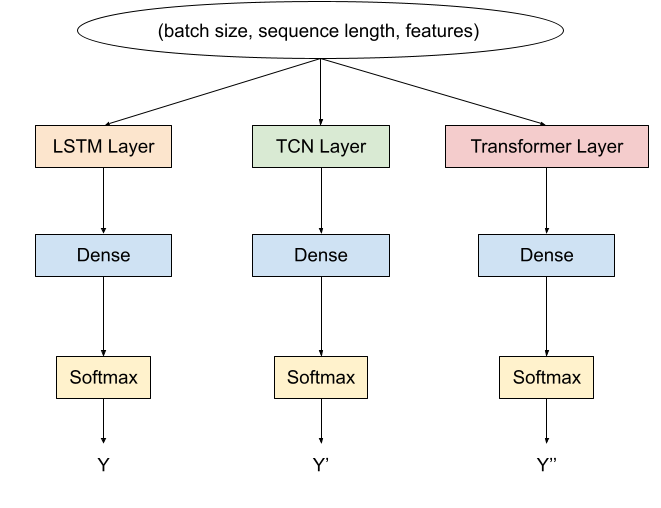
\includegraphics[width=\textwidth]{cap4/architectures.png}
    \caption{Diagrams of architectures in analysis}
    \label{fig:architectures}
\end{figure}

\hfill \break
Figure \ref{fig:architectures} describes how the three architectures in analysis, namely LSTM, TCN, and Transformers, were used. We can think of the three architectures as a building block of a more common architecture for generating allocations. Indeed one can notice in the figure before mentioned a certain degree of similarity. We can abstract and see the three architectures nothing more than another layer of an architecture. Now, we define an architecture were: \begin{itemize}
\item The input is a vector $x \in \mathbb{R}^3$ with dimension $(b \times s \times f)$ where $b$ is the batch size, $s$ is the sequence length and $f$ the number of features
\item the first layer is a parameter, than can be either an LSTM, TCN or Transformer layer.
\item Since each architecture have a different internal dimension their output dimension is different so we add now a Dense layer with output dimension four. This add another level of expressivity to our architecture.

\item It is not guaranteed that the output values of the Dense layer are a weight vector that sum up to one. Therefore, as Zhang \cite{Zhang_2020} does, in all the tested models the last layer is always a \textit{softmax} layer. A softmax layer is a layer that implements the softmax function:

$$ softmax(\bar{x}) = \frac{e^{\bar{x}}}{\Sigma_{i=0}^n e^{\bar{x}_i}}  $$

This is often used to to normalize the output of a network to a probability distribution or as in our case to normalize values as allocation weights, to force them sum up to one.

\end{itemize}

\hfill \break

Entering more in details into the architectures, LSTM is as described in section \ref{lstm_section} with specific parameters the number of units and the number of LSTM layers. TCNs is as described in section \ref{tcn_section} with temporal dilated convolution and residual connection. The Transformer architecture used is the regression transformer described in section \ref{transformers_section} with residual connections, layer normalization and dropout. Table \ref{table:archi_hyper} list all hyperparameters of the architectures in consideration. 

\begin{table}[h]
\resizebox{\textwidth}{!}{%
\begin{tabular}{lll}
Model / method                                             & Parameter & Description                      \\ \hline
\multicolumn{1}{c}{\multirow{4}{*}{Common to all methods}} & b         & Training bath size               \\
\multicolumn{1}{c}{}                                       & e         & Training epochs                  \\
\multicolumn{1}{c}{}                                       & lr        & Learning rate                    \\
\multicolumn{1}{c}{}                                       & s         & sequence lenght                  \\ \hline
\multirow{2}{*}{LSTM}                                      & d         & internal/hidden dimension, units \\
                                                           & l         & numer of layers                  \\ \hline
\multirow{4}{*}{TCN}                                       & d         & internal/hidden dimension, units \\
                                                           & l         & numer of layers                  \\
                                                           & k         & kernel size                      \\
                                                           & sk        & residual connections (Yes/No)    \\ \hline
\multirow{4}{*}{Transformer}                               & h         & number of attention heads        \\
                                                           & hd        & internal/hidden dimension, units \\
                                                           & o         & output dimension                 \\
                                                           & l         & number of layers                
\end{tabular}%
}
\caption{Architecture hyperparameters \label{table:archi_hyper}}
\end{table}


\hfill

When searching for a model in machine learning, the problem is essentially about finding the proper input data, architecture and hyperparameters. Each of these has an impact on the others. This means that changing one parameter or component may result in another parameter or component no longer being the best option. The safest choice would be doing a grid search, trying all the possibilities to find the best combination that maximize performance. However, this is often not possible for time and performance reasons. In this work we followed an order of operation that first select the most critical parameters and then fine tuning less impactful one, in an iterating manner, as follows:
\begin{enumerate}
    \item We started only with daily returns as input features, because is a small feature set that allows us to experiment quickly and is the base feature from which all others features are generated. Technically every network could generate all the other features from returns, so this input feature is an adequate starting point.
    \item As hyperparameters we started with batch size 100, learning rate $10^{-2}$ and sequence length $256$ and $5$ epochs. 
    \item We started using the TCN to find out which features were the most useful and had greater impact.
    \item Then hyperparameters like learning rate, batch size and epochs were corrected without changing inputs features and architecture.
    \item Then with the new  hyperparameters, we try different architectures.
    \item Lastly, fine tuning hyperparameters is again performed, especially the one of the architecture.
\end{enumerate}

\hfill \break

We applied several techniques of \textbf{holdout validation}. Initially the training period was 2013-2018 with 2019-2020 as validation set. But in 2020 the market was in a very special phase, caused by the COVID-19 pandemic and the March 2020 stock markets crash. This caused that networks outperforms in the validation set because they are not trained for a very bear market and the rapid recovery that happened afterward. The model was suffering from high variance (see Chapter \ref{CH:theoryML}).
3-fold validation is then used and specifically:
\begin{itemize}
    \item Training on 2013-2018 and validation on 2019-2020
    \item Training on 2015-2020 and validation on 2013-2014
    \item Training on external periods 2013-2015, 2018-2020 and validation on the middle period 2016-2017
\end{itemize}
In this way we select models that are overall satisfactory in the most preponderant market phases. In each period the model is re-initialized twice and trained twice. The results are averaged. The same is done for the results of all periods for having an indicative, general across-dataset metric. This is done for avoiding considering wrong models where the model learn the wrong general function, but that is instead good for a specific case. For example the allocation $1/n$ is extremely easy to learn, good in many situations (see \cite{PFLUG2012410} \cite{demiguel2009} \cite{duchin2009markowitz}) but not in all.

\hfill \break

All the models have been implemented in open-source machine learning framework TensorFlow \cite{tensorflow2015-whitepaper}. Development has been carried out using Jupyter Notebooks \cite{Kluyver2016jupyter}, as they allow a faster visualization of results.


\section{Sharpe ratio maximizing model}
\label{s:sharpe_maximizing_model}

As in \textit{Zhang et al. (2020)} \cite{Zhang_2020}, an inverted \textbf{Sharpe ratio maximizing function} has been initially used. The function calculates the Sharpe ratio of the portfolio with the weights produced by the network. The code of the loss function can be found on the listing \ref{lst:sharpe_ratio} .


\begin{figure}[h]
\begin{lstlisting}[language=Python, caption=Python function to compute the portfolio sharpe given new assets weights from neural network, label=lst:sharpe_ratio,frame = single]
@tf.function
def sharpe(output, past_data, past_weights, today_data):
    # expected return / std dev of porfolio
    # get returns from today_data
    # multiply with network choosed weight
    weighted_returns = tf.multiply(output,today_data)
    # get comulated return of last period
    past_returns = past_data
    weighted_past_returns = past_returns*past_weights
    cumulative = tf.math.reduce_prod(
        (1+weighted_past_returns)
        ,axis=0)
    # mutiply today data with cumulative from past
    total = (cumulative * (weighted_returns+1))-1
    # std_dev of last period
    weighted_past_returns =
        tf.squeeze(weighted_past_returns)
    std_dev = tf.concat(
        [weighted_past_returns,weighted_returns]
        ,axis=0)
    std_dev = tf.math.reduce_std(std_dev,axis=0)
    # ratio
    sharpe = total/std_dev
    return tf.math.reduce_mean(sharpe)
\end{lstlisting}
\end{figure}


The Sharpe ratio sign is then inverted to minimize it.
Weights produced by the network are saved in a temporary array in a FIFO data buffer manner to be used for next Sharpe ratio computations.
The Sharpe computation is made inside a context of automatic differentiation thought GradientTape API. After this, gradients are explicitly computed and applied.

\hfill \break

A normalization layer had to be implemented, to force the model to output weights that are between the 5\% and 60\% chosen bound, as specified in the section \ref{s:research_objective}. This is because maximizing Sharpe ratio does not guarantee the allocation weights will be contained in that range. This normalization layer has been implemented directly as a Keras layer, instead of normalizing the weights after they have been generated from the network. This is to enforce the loss to be computed on correct and operational weights, to constrain the model to learn to produce an allocation we can use in our scenario. The code of the normalization layer can be seen in the listings \ref{lst:normalization_layer} and is inspired by the following formula:
$$(t_{max} - t_{min}) - \frac{m-r_{min}}{r_{max}-r_{min}} + t_{min}$$


\begin{minipage}{\textwidth}
Where:
\begin{itemize}
    \item $m$ is the value to be scaled
    \item $r_{min}$ minimum in the range of values
    \item $r_{max}$ maximum in the range of values
    \item $t_{min}$ minimum in the desired target scaling
    \item $t_{max}$ maximum in the desired target scaling
\end{itemize}
\end{minipage}




\begin{minipage}{\linewidth}
\begin{lstlisting}[language=Python, caption=Keras layer to force the weights to be between 5\% and 60\%, label=lst:normalization_layer, frame = single]
min_bound = 0.05
max_bound = 0.6
def normalization_layer(x):
    minV = tf.repeat(tf.expand_dims(
        keras.layers.Minimum()(tf.unstack(x,4,axis=-1))
        ,axis=1),4,axis=-1)
    maxV =  tf.repeat(tf.expand_dims(
        keras.layers.Maximum()(
            tf.unstack(x,4,axis=-1))
        ,axis=1),4,axis=-1)
    return (max_bound-min_bound)
                *((x-minV)/(maxV-minV))+min_bound
\end{lstlisting}
\end{minipage}


\section{Target allocation matching model}
\label{s:target_allocation_model}

Next, a different type of model was tested. Instead of maximising the Sharpe ratio we use a network which still generates weights but the loss function is the mean squared error (MSE) between these generated weights and some optimal weights.
Formally, given the vector $w = [w_1, w_2, w_3, w_4]$ generated by the network and the vector $y= [y_1, y_2, y_3, y_3]$ of the target allocation, we define the MSE loss in this context as:
$$ MSE(w,y) = \frac{1}{4} \sum_{i=1}^4 (y_i - w_i)^2  $$
In this example we used four as number of assets but this definition can be easily extended to any number of assets.

\hfill \break

The optimal weights are generated for the training set through an algorithm with knowledge of future returns. This algorithm can make use of Markowitz optimization (see chapter \ref{CH:theoryFI} and PyPortfolioOpt in the Appendix) or other basic algorithms like the following one:

\begin{algorithm}[h]
\caption{Caption}
\label{alg1}
\begin{algorithmic}
\item Order assets comulated returns in a window in decreasing order. 
\item Assign respectively 40\%, 30\%, 20\%, 10\% to the first, second, third and forth asset.

\end{algorithmic}
\end{algorithm}


\section{Reproducibility}
\label{s:reproducibility}
An experiment is \textbf{reproducible} when it can be executed multiple times and obtain the same result. In the context of machine learning this is not easy to achieve. Framework like Keras have several random initialization, especially of network layer kernels. The reason is to increase the likelihood of starting exploring the parameter space in a gradient slope and increase the possibility of convergence. But to obtain reproducibility, it is then suggested to initialize the weights to the same value and if not possible to initialize their random generator to the same initial seed.

\hfill \break

Reproducibility is an  important aspect of this work especially when in the phase where different features sets were tested. Once a feature set was discovered to be upstanding with respect to the others, it was run on a fresh copy of the model to verify the results. But by default TensorFlow resets the kernels and other parameters every time to random values. It was then necessary to fix the random seed to a fixed value in each notebook. Moreover, the kernel of each layer has been initialized to a unit value for the first layers of each model, and to a normal distribution but with unit seed for the fully connected last layer. Initializing the last layer to a unit value was not guaranteeing convergence. This effectively improved the reproducibility of the results.

\section{Fixed allocation anomaly}
\label{s:fixed_allocation_anomaly}

The weights generated by the network, with both loss function methods, initially had the problem of being fixed even as the inputs changed. This can be seen in the right part of plot \textit{a} in figure \ref{fig:with_without_bias}. Allocation weights change during training but they remain the last computed by the backpropagation algorithm in the last iteration of the training algorithm. During training they change only because the internal weights of the network change, but in validation when the internal weights are not allowed to change, also the output remain fixed. 

\begin{figure}[h]
    \centering
    \subfloat[\centering Not optimal allocation, is fixed in testing period]{{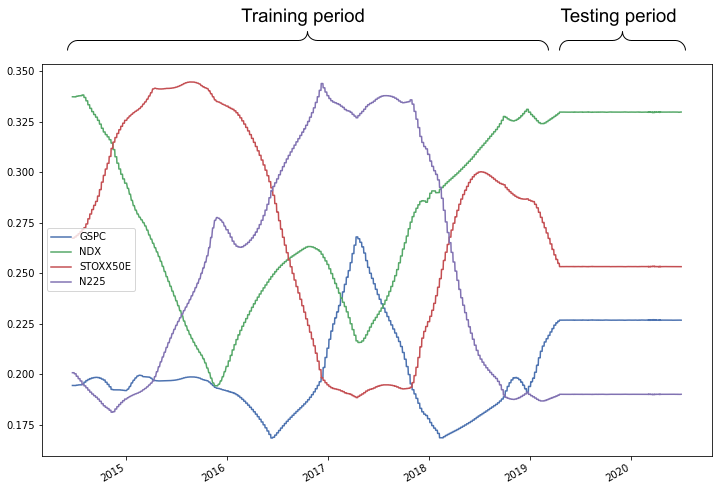
\includegraphics[width=0.9\textwidth]{cap4/Fixed_allocation_annotated.png} }}%
    \qquad
    \subfloat[\centering  optimal allocation, is dynamic in both train and test dataset ]{{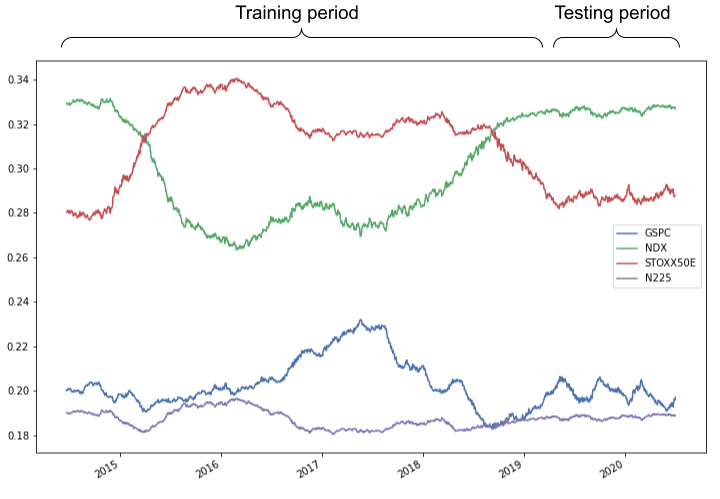
\includegraphics[width=0.9\textwidth]{cap4/Dynamic Allocation annotated.png} }}%
    \caption[Fixed allocation anomaly]{Fixed and not-fixed allocations}%
    \label{fig:with_without_bias}%
\end{figure}

\hfill \break

The reason of this phenomenon is that the network only found the best bias value to increase the overall performance, both in terms of Sharpe ratio or of return. The input weights are null, that means the network does not use the input features to compute the output. 
\hfill \break

Although the performance on the validation dataset was indeed good on the first days, because it fitted the market phase of the last period of training set, it degraded over time. This was the case the validation set was temporally right after the training set, in the different cases the fixed allocation resulted in a bad performance from the very beginning.  In general, this was a case when the training algorithm was stopped in a local minimum, the network found out how to minimize the target loss but did not find a relationship between input and optimal outputs.

\hfill \break

\begin{figure}[H]
    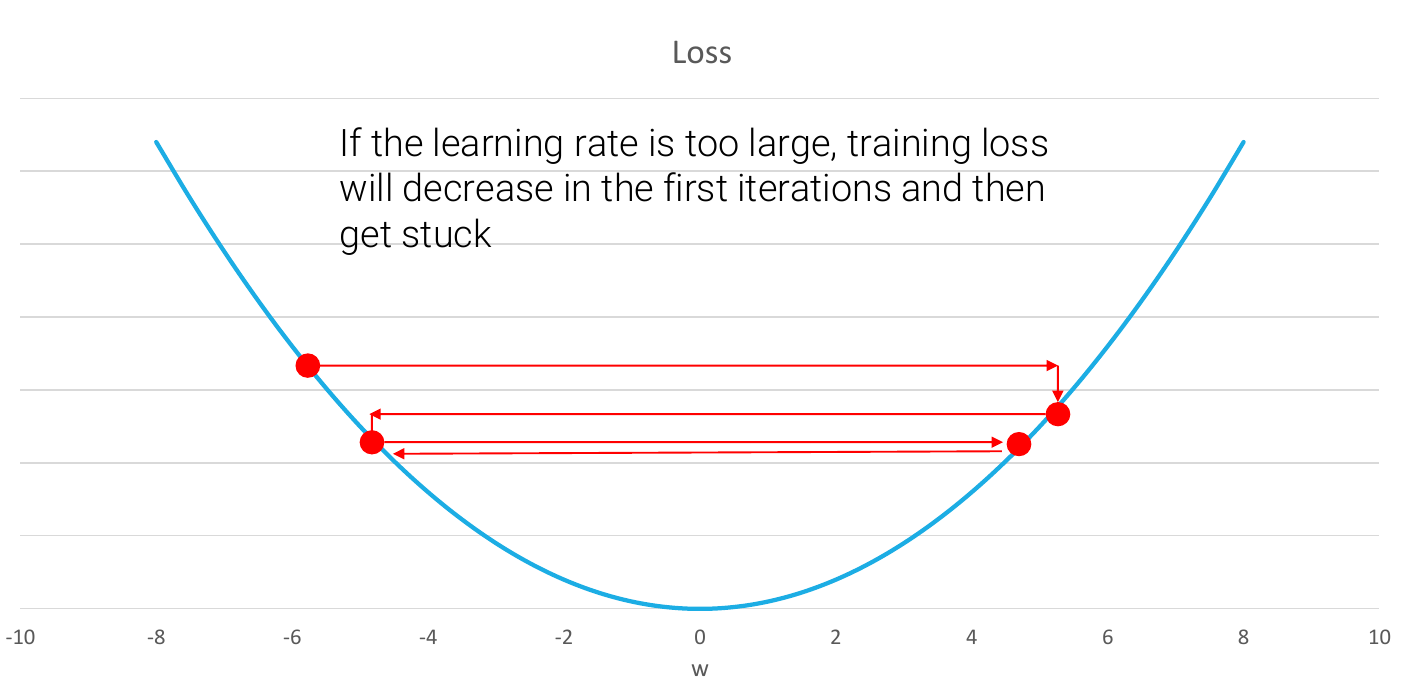
\includegraphics[width=12cm]{cap4/too_large_lr.png}
    \caption[Excessive learning rate effects]{Excessive learning rate effects \cite{salti_cv} }
    \label{fig:too_lage_lr}
\end{figure}

Most of the time, this situation was solved by reducing the learning rate.
\textbf{Learning rate} is a fundamental hyperparameter. A too large learning rate, while it can make convergence faster, increases the likelihood of the training getting trapped in an oscillation like shown in figure \ref{fig:too_lage_lr}. Instead, a too small learning rate makes training too slow and the algorithm could convergence very late or never converge if not enough training time is provided.

The initial learning rate of $10^{-2}$ was changed to $10^{-3}$  with radical changes in the output quality. In this case the gradient was persisting in an oscillatory state in a  in the parameters space, finding a sub-optimal solution changing bias value and ignoring input values. By lowering the learning rate and increasing the number of epochs, the gradient would slowly direct the training to a state where inputs were effectively used and a more optimal portfolio allocation was found.

\hfill \break

In cases were lowering the learning rate was not sufficient, we resorted to force \textbf{constraints on the biases} of each layer by using the constraint \texttt{max\_norm(0)} provided by TensorFlow. This forces the network to use the inputs for providing the output and effectively finding a relation between them.
In the figure \ref{fig:with_without_bias} we see the difference in computed allocation weight by a fixed situation and a dynamic one. 



\section{Remaining hyperparameters}
\label{s:remaining_hyperparameters}

Batch size was initially set to a value of 100. With time we noticed that a smaller batch size, for example of value 5, was better. The reason is the following. The value of the loss function is averaged always across the batch size. A too large batch size makes the loss value too general and uniform across the training. The result is that some micro-variations in the market of the duration of few days are lost and the network is not learning how to react and take advantage of them. On the opposite situation, having a batch size too small, for example only one sample, is disadvantageous. This is because the network would pay too attention in the inherent noise that is inside a market and would be unable to highlight weekly trend. The gradient would change direction contentiously from sample to sample, unable to find a common minimum in the parameter space.
 It must be considered that even if the time frame is not negligible this is not a high trading frequency application as many others in this field and only daily data is available. This makes the dataset considerably small with respect to other machine learning applications. It is therefore essential to have have a reduced batch size.

\hfill \break

Experiments with different windows size have been carried out. A smaller window size allows the model to react faster to sudden market phase change while a longer window allows the model to understand long-term factors and implication in the market and invest in more stable assets.







